\documentclass[12pt]{article}

\usepackage[a4paper,left=1cm,right=1cm,top=1.5cm,bottom=1.5cm]{geometry}
\usepackage[T1]{fontenc}
\usepackage[utf8]{inputenc}
\usepackage{lmodern}
\usepackage{amsmath}
\usepackage{amssymb}
\usepackage{array}
\usepackage{graphicx}
\usepackage{adjustbox}
\usepackage{multicol}
\usepackage{enumitem}
\usepackage{tikz}

\usetikzlibrary{arrows.meta}

\setlength{\parindent}{0pt}
\setlength{\parskip}{0pt}
\setlength{\columnsep}{0.7cm}
\setlength{\columnseprule}{0.4pt}
\renewcommand{\arraystretch}{1.35}

\newcommand{\QuestionMarks}[1]{\hfill [#1]}
\newcommand{\AnswerLine}[1]{\makebox[#1]{\hrulefill}}
\newcommand{\AnswerBox}{\fbox{\rule{0pt}{0.8cm}\rule{0.8cm}{0pt}}}
\newcommand{\FractionAnswerBox}{\fbox{\rule{0pt}{0.55cm}\rule{0.55cm}{0pt}}}

\newcommand{\BoxedQuestionLabel}[1]{%
	\begingroup
	\setlength{\fboxsep}{0pt}%
	\raisebox{-0.12cm}{%
		\fbox{%
			\makebox[0.68cm][c]{\rule[-0.18cm]{0pt}{0.68cm}\textbf{#1}}%
		}%
	}%
	\endgroup
}

\begin{document}
	\raggedcolumns
	\begin{multicols}{2}
		\begin{enumerate}[
			label=\BoxedQuestionLabel{\arabic*},
			leftmargin=1.1cm,
			labelwidth=0.72cm,
			labelsep=0.25cm,
			itemsep=0pt,
			topsep=0pt,
			parsep=0pt
			]
			
			\item
			Complete the sentence.
			
			\vspace{0.45cm}
			
			The value of the digit 3 in 3\,451 is
			\hfill \AnswerLine{4.6cm} \QuestionMarks{1}
			
			\vspace{0.85cm}
			
			\item
			Draw a ring around all the multiples of 2.
			
			\vspace{0.65cm}
			
			\[
			889
			\qquad\qquad
			120
			\qquad\qquad
			465
			\qquad\qquad
			351
			\qquad\qquad
			296
			\]
			
			\vspace{0.35cm}
			
			\QuestionMarks{1}
			
			\vspace{0.95cm}
			
			\item
			Write a number in each box to complete the sentences.
			
			\vspace{0.65cm}
			
			\[
			\frac{4}{5}
			\quad + \quad
			\frac{2}{5}
			\quad = \quad
			\frac{\FractionAnswerBox}{\FractionAnswerBox}
			\]
			
			\vspace{0.95cm}
			
			\[
			\frac{8}{10}
			\quad - \quad
			\frac{3}{10}
			\quad = \quad
			\frac{\FractionAnswerBox}{\FractionAnswerBox}
			\]
			
			\vspace{0.35cm}
			
			\QuestionMarks{2}
			
			\vspace{0.8cm}
			
			\item
			Draw a ring around all the 2D shapes with a perimeter of 8 cm.
			
			\vspace{0.35cm}
			
			\begin{center}
				\begin{adjustbox}{max width=\linewidth}
					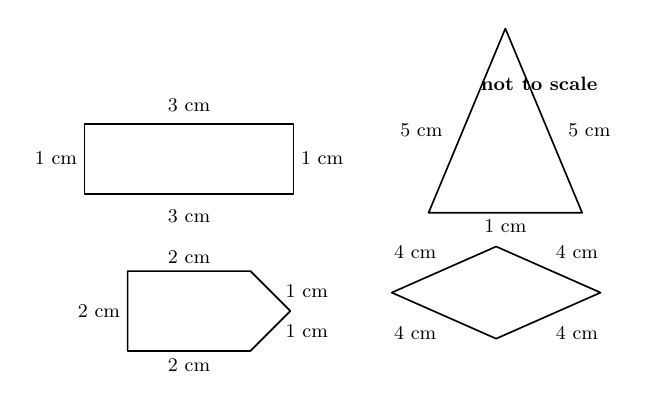
\begin{tikzpicture}[
						scale=0.78,
						every node/.style={font=\small, transform shape},
						line cap=round,
						line join=round
						]
						
						\node at (7.4,4.35) {\textbf{not to scale}};
						
						% Top-left rectangle: 3 cm by 1 cm
						\begin{scope}[shift={(0,2.55)}]
							\draw[line width=0.6pt] (0,0) rectangle (3.4,1.15);
							\node at (1.7,1.45) {3 cm};
							\node at (1.7,-0.35) {3 cm};
							\node[left] at (0,0.58) {1 cm};
							\node[right] at (3.4,0.58) {1 cm};
						\end{scope}
						
						% Top-right triangle
						\begin{scope}[shift={(5.6,2.25)}]
							\draw[line width=0.6pt] (0,0) -- (1.25,3.0) -- (2.5,0) -- cycle;
							\node[left] at (0.35,1.35) {5 cm};
							\node[right] at (2.15,1.35) {5 cm};
							\node[below] at (1.25,0) {1 cm};
						\end{scope}
						
						% Bottom-left pentagon
						\begin{scope}[shift={(0.7,0)}]
							\draw[line width=0.6pt]
							(0,0) -- (2.0,0) -- (2.65,0.65) -- (2.0,1.3) -- (0,1.3) -- cycle;
							\node[above] at (1.0,1.3) {2 cm};
							\node[below] at (1.0,0) {2 cm};
							\node[left] at (0,0.65) {2 cm};
							\node[right] at (2.45,0.98) {1 cm};
							\node[right] at (2.45,0.32) {1 cm};
						\end{scope}
						
						% Bottom-right rhombus
						\begin{scope}[shift={(5.0,0.2)}]
							\draw[line width=0.6pt] (0,0.75) -- (1.7,1.5) -- (3.4,0.75) -- (1.7,0) -- cycle;
							\node[above left] at (0.85,1.18) {4 cm};
							\node[above right] at (2.55,1.18) {4 cm};
							\node[below left] at (0.85,0.32) {4 cm};
							\node[below right] at (2.55,0.32) {4 cm};
						\end{scope}
						
					\end{tikzpicture}
				\end{adjustbox}
			\end{center}
			
			\vspace{0.2cm}
			
			\QuestionMarks{1}
			
			\vspace{0.8cm}
			
			\item
			Here is a rectangle drawn on a grid of squares.
			
			\vspace{0.35cm}
			
			\begin{center}
				\begin{adjustbox}{max width=\linewidth}
					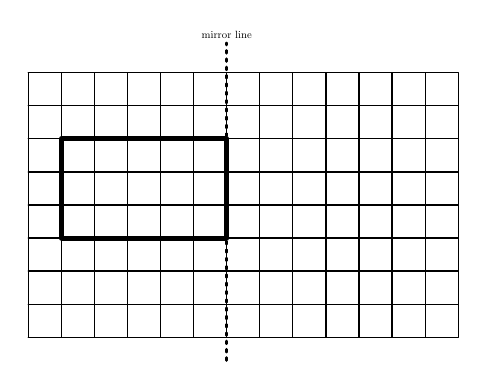
\begin{tikzpicture}[
						scale=0.42,
						every node/.style={font=\small, transform shape},
						line cap=round,
						line join=round
						]
						
						% Grid
						\draw[step=1, line width=0.45pt] (0,0) grid (13,8);
						
						% Rectangle
						\draw[line width=1.8pt] (1,3) rectangle (6,6);
						
						% Mirror line
						\draw[dotted, line width=1pt] (6,-0.7) -- (6,8.9);
						\node[above] at (6,8.9) {mirror line};
						
					\end{tikzpicture}
				\end{adjustbox}
			\end{center}
			
			\vspace{0.35cm}
			
			Draw the reflection of the rectangle in the mirror line. \QuestionMarks{1}
			
			\vspace{0.8cm}
			
			\item
			Write the number that can be expressed as
			
			\vspace{0.35cm}
			
			\[
			90\,000
			\quad + \quad
			2\,000
			\quad + \quad
			500
			\quad + \quad
			40
			\quad + \quad
			6
			\]
			
			\vspace{0.45cm}
			
			\hfill \AnswerLine{4.2cm} \QuestionMarks{1}
			
			\vspace{0.9cm}
			
			\item
			Here are the spatial patterns for some square numbers.
			
			\vspace{0.35cm}
			
			\begin{center}
				\begin{adjustbox}{max width=\linewidth}
					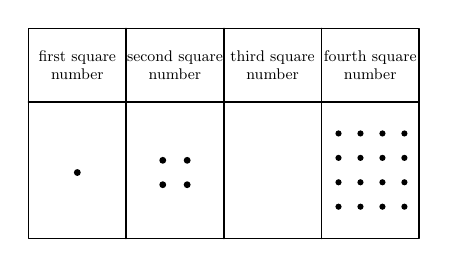
\begin{tikzpicture}[
						scale=0.62,
						every node/.style={font=\small, transform shape},
						line cap=round,
						line join=round
						]
						
						% Table border and grid
						\draw[line width=0.6pt] (0,0) rectangle (8,4.3);
						\draw[line width=0.6pt] (2,0) -- (2,4.3);
						\draw[line width=0.6pt] (4,0) -- (4,4.3);
						\draw[line width=0.6pt] (6,0) -- (6,4.3);
						\draw[line width=0.6pt] (0,2.8) -- (8,2.8);
						
						% Headings
						\node[align=center] at (1,3.55) {first square\\number};
						\node[align=center] at (3,3.55) {second square\\number};
						\node[align=center] at (5,3.55) {third square\\number};
						\node[align=center] at (7,3.55) {fourth square\\number};
						
						% First square number: 1
						\fill (1,1.35) circle (2pt);
						
						% Second square number: 4
						\foreach \x in {2.75,3.25}
						\foreach \y in {1.10,1.60}
						\fill (\x,\y) circle (2pt);
						
						% Third square number left blank for the student
						
						% Fourth square number: 16
						\foreach \x in {6.35,6.80,7.25,7.70}
						\foreach \y in {0.65,1.15,1.65,2.15}
						\fill (\x,\y) circle (1.8pt);
						
					\end{tikzpicture}
				\end{adjustbox}
			\end{center}
			
			\vspace{0.25cm}
			
			Draw the spatial pattern for the third square number. \QuestionMarks{1}
			
			\vspace{0.85cm}
			
			\item
			Calculate.
			
			\vspace{0.65cm}
			
			\hspace*{1.6cm}
			\(83 \times 100\)
			\hfill \AnswerLine{4.0cm}
			
			\vspace{1.25cm}
			
			\hspace*{1.6cm}
			\(52\,300 \div 100\)
			\hfill \AnswerLine{4.0cm} \QuestionMarks{1}
			
			\vspace{0.8cm}
			
			\item
			Here are some 2D shapes and 3D objects.
			
			\vspace{0.25cm}
			
			Each 2D shape folds to make one of the 3D objects.
			
			\vspace{0.25cm}
			
			\begin{center}
				\begin{adjustbox}{max width=\linewidth}
					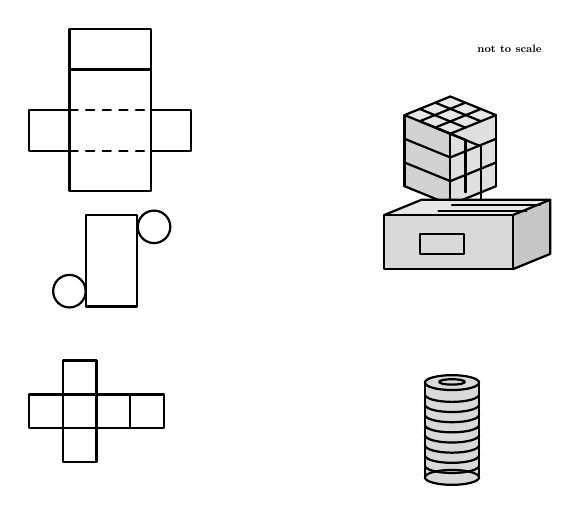
\begin{tikzpicture}[
						line cap=round,
						line join=round,
						draw=black,
						thick,
						fold/.style={dashed, thick},
						scale=0.43,
						every node/.style={font=\small, transform shape}
						]
						
						\node at (14.2,10.2) {\textbf{not to scale}};
						
						% Rectangular prism net
						\begin{scope}[shift={(0,7.2)}]
							\draw (1.2,-1.2) rectangle (3.6,2.4);
							\draw (0,0) rectangle (1.2,1.2);
							\draw (3.6,0) rectangle (4.8,1.2);
							\draw (1.2,2.4) rectangle (3.6,3.6);
							
							\draw[fold] (1.2,0) -- (3.6,0);
							\draw[fold] (1.2,1.2) -- (3.6,1.2);
							\draw[fold] (1.2,2.4) -- (3.6,2.4);
							\draw[fold] (1.2,0) -- (1.2,1.2);
							\draw[fold] (3.6,0) -- (3.6,1.2);
						\end{scope}
						
						% Cylinder net
						\begin{scope}[shift={(0.7,2.6)}]
							\draw (1,0) rectangle (2.5,2.7);
							\draw (0.5,0.45) circle (0.48);
							\draw (3.0,2.35) circle (0.48);
						\end{scope}
						
						% Cube net
						\begin{scope}[shift={(0,-1)}]
							\foreach \x in {0,1,2,3}
							\draw (\x,0) rectangle ++(1,1);
							
							\draw (1,1) rectangle ++(1,1);
							\draw (1,-1) rectangle ++(1,1);
							
							\draw[fold] (1,0) -- (1,1);
							\draw[fold] (2,0) -- (2,1);
							\draw[fold] (3,0) -- (3,1);
							\draw[fold] (1,1) -- (2,1);
							\draw[fold] (1,0) -- (2,0);
						\end{scope}
						
						% Cube with visible square grid
						\begin{scope}[shift={(11.1,8.25)}]
							\coordinate (A) at (0,0);
							\coordinate (B) at (1.35,0.55);
							\coordinate (C) at (2.70,0);
							\coordinate (D) at (1.35,-0.55);
							\coordinate (E) at (0,-2.1);
							\coordinate (F) at (1.35,-2.65);
							\coordinate (G) at (2.70,-2.1);
							
							\fill[gray!18] (A) -- (B) -- (C) -- (D) -- cycle;
							\fill[gray!35] (A) -- (D) -- (F) -- (E) -- cycle;
							\fill[gray!25] (D) -- (C) -- (G) -- (F) -- cycle;
							
							\draw (A) -- (B) -- (C) -- (D) -- cycle;
							\draw (A) -- (E);
							\draw (D) -- (F);
							\draw (C) -- (G);
							\draw (E) -- (F) -- (G);
							
							% top grid
							\draw (0.45,0.18) -- (1.80,-0.37);
							\draw (0.90,0.37) -- (2.25,-0.18);
							\draw (0.45,-0.18) -- (1.80,0.37);
							\draw (0.90,-0.37) -- (2.25,0.18);
							
							% left face grid
							\draw (0.45,-0.18) -- (1.80,-0.73);
							\draw (0.90,-0.37) -- (2.25,-0.92);
							\draw (0,-0.70) -- (1.35,-1.25);
							\draw (0,-1.40) -- (1.35,-1.95);
							
							% right face grid
							\draw (1.80,-0.73) -- (1.80,-2.28);
							\draw (2.25,-0.92) -- (2.25,-2.47);
							\draw (1.35,-1.25) -- (2.70,-0.70);
							\draw (1.35,-1.95) -- (2.70,-1.40);
						\end{scope}
						
						% Rectangular prism
						\begin{scope}[shift={(10.5,3.7)}]
							\coordinate (A) at (0,0);
							\coordinate (B) at (3.8,0);
							\coordinate (C) at (3.8,1.6);
							\coordinate (D) at (0,1.6);
							\coordinate (E) at (1.1,0.45);
							\coordinate (F) at (4.9,0.45);
							\coordinate (G) at (4.9,2.05);
							\coordinate (H) at (1.1,2.05);
							
							\fill[gray!30] (A)--(B)--(C)--(D)--cycle;
							\fill[gray!45] (B)--(F)--(G)--(C)--cycle;
							\fill[gray!18] (D)--(C)--(G)--(H)--cycle;
							
							\draw (A)--(B)--(C)--(D)--cycle;
							\draw (B)--(F)--(G)--(C);
							\draw (D)--(H)--(G);
							
							\draw (1.05,0.45) rectangle (2.35,1.05);
							\draw (1.6,1.72) -- (4.2,1.72);
							\draw (2.0,1.9) -- (4.6,1.9);
						\end{scope}
						
						% Cylinder
						\begin{scope}[shift={(12.5,0.35)}]
							\def\rx{0.8}
							\def\ry{0.22}
							\def\h{2.8}
							
							\fill[gray!30] (-\rx,0) -- (-\rx,-\h) arc[start angle=180,end angle=360,x radius=\rx,y radius=\ry] -- (\rx,0) arc[start angle=0,end angle=180,x radius=\rx,y radius=\ry];
							
							\draw (0,0) ellipse[x radius=\rx,y radius=\ry];
							\draw (-\rx,0) -- (-\rx,-\h);
							\draw (\rx,0) -- (\rx,-\h);
							\draw (0,-\h) ellipse[x radius=\rx,y radius=\ry];
							
							\foreach \y in {-0.35,-0.65,-0.95,-1.25,-1.55,-1.85,-2.15,-2.45}
							\draw (-\rx,\y) arc[start angle=180,end angle=360,x radius=\rx,y radius=\ry];
							
							\draw (0,0.02) ellipse[x radius=0.38,y radius=0.08];
						\end{scope}
						
					\end{tikzpicture}
				\end{adjustbox}
			\end{center}
			
			\vspace{0.35cm}
			
			Draw a line to match each 2D shape to the 3D object it folds to make. \QuestionMarks{1}
			
			\vspace{0.8cm}
			
			\item
			\textbf{(a)}\quad Calculate.
			
			\vspace{0.35cm}
			
			\[
			453 - 134
			\]
			
			\vspace{0.45cm}
			
			\hfill \AnswerLine{4.2cm} \QuestionMarks{1}
			
			\vspace{0.8cm}
			
			\hspace*{0.2cm}
			\textbf{(b)}\quad
			An aeroplane flies from London to Dubai and then flies from Dubai to Sydney.
			
			\vspace{0.35cm}
			
			\begin{center}
				\begin{adjustbox}{max width=\linewidth}
					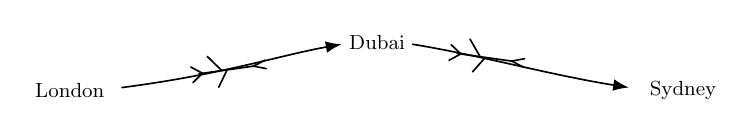
\begin{tikzpicture}[
						scale=0.82,
						every node/.style={font=\small, transform shape},
						line cap=round,
						line join=round
						]
						
						\node[anchor=east] at (0,0) {London};
						\node at (4.1,0.75) {Dubai};
						\node[anchor=west] at (8.2,0) {Sydney};
						
						\draw[-{Latex[length=2mm]}, line width=0.6pt]
						(0.15,0.05) .. controls (1.7,0.25) and (2.6,0.55) .. (3.55,0.72);
						
						\draw[-{Latex[length=2mm]}, line width=0.6pt]
						(4.65,0.72) .. controls (5.7,0.55) and (6.75,0.25) .. (8.0,0.05);
						
						% First aeroplane
						\begin{scope}[shift={(1.75,0.32)}, rotate=8, scale=0.55]
							\draw[line width=0.6pt] (-0.75,0) -- (0.8,0);
							\draw[line width=0.6pt] (0.8,0) -- (1.15,0.12);
							\draw[line width=0.6pt] (0.8,0) -- (1.15,-0.12);
							\draw[line width=0.6pt] (-0.1,0) -- (-0.45,0.45);
							\draw[line width=0.6pt] (0.05,0) -- (-0.25,-0.45);
							\draw[line width=0.6pt] (-0.65,0) -- (-0.95,0.22);
							\draw[line width=0.6pt] (-0.65,0) -- (-0.95,-0.22);
						\end{scope}
						
						% Second aeroplane
						\begin{scope}[shift={(5.75,0.52)}, rotate=-8, scale=0.55]
							\draw[line width=0.6pt] (-0.75,0) -- (0.8,0);
							\draw[line width=0.6pt] (0.8,0) -- (1.15,0.12);
							\draw[line width=0.6pt] (0.8,0) -- (1.15,-0.12);
							\draw[line width=0.6pt] (-0.1,0) -- (-0.45,0.45);
							\draw[line width=0.6pt] (0.05,0) -- (-0.25,-0.45);
							\draw[line width=0.6pt] (-0.65,0) -- (-0.95,0.22);
							\draw[line width=0.6pt] (-0.65,0) -- (-0.95,-0.22);
						\end{scope}
						
					\end{tikzpicture}
				\end{adjustbox}
			\end{center}
			
			\vspace{0.35cm}
			
			420 passengers get on an empty plane in London.
			
			96 passengers get off the plane in Dubai.
			
			52 new passengers get on the plane in Dubai.
			
			\vspace{0.45cm}
			
			Calculate the number of passengers on the plane when it arrives in Sydney.
			
			\vspace{0.75cm}
			
			\hfill \AnswerLine{4.2cm}\quad passengers \QuestionMarks{1}
			
			\vspace{0.8cm}
			
			\item
			\textbf{(a)}\quad Calculate.
			
			\vspace{0.35cm}
			
			\[
			453 - 134
			\]
			
			\vspace{0.45cm}
			
			\hfill \AnswerLine{4.2cm} \QuestionMarks{1}
			
			\vspace{0.8cm}
			
			\hspace*{0.2cm}
			\textbf{(b)}\quad
			An aeroplane flies from London to Dubai and then flies from Dubai to Sydney.
			
			\vspace{0.35cm}
			
			\begin{center}
				\begin{adjustbox}{max width=\linewidth}
					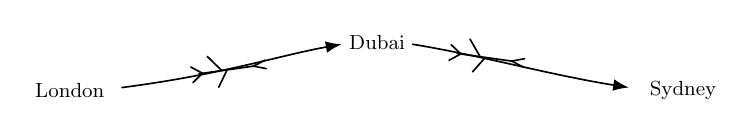
\begin{tikzpicture}[
						scale=0.82,
						every node/.style={font=\small, transform shape},
						line cap=round,
						line join=round
						]
						
						\node[anchor=east] at (0,0) {London};
						\node at (4.1,0.75) {Dubai};
						\node[anchor=west] at (8.2,0) {Sydney};
						
						\draw[-{Latex[length=2mm]}, line width=0.6pt]
						(0.15,0.05) .. controls (1.7,0.25) and (2.6,0.55) .. (3.55,0.72);
						
						\draw[-{Latex[length=2mm]}, line width=0.6pt]
						(4.65,0.72) .. controls (5.7,0.55) and (6.75,0.25) .. (8.0,0.05);
						
						% First aeroplane
						\begin{scope}[shift={(1.75,0.32)}, rotate=8, scale=0.55]
							\draw[line width=0.6pt] (-0.75,0) -- (0.8,0);
							\draw[line width=0.6pt] (0.8,0) -- (1.15,0.12);
							\draw[line width=0.6pt] (0.8,0) -- (1.15,-0.12);
							\draw[line width=0.6pt] (-0.1,0) -- (-0.45,0.45);
							\draw[line width=0.6pt] (0.05,0) -- (-0.25,-0.45);
							\draw[line width=0.6pt] (-0.65,0) -- (-0.95,0.22);
							\draw[line width=0.6pt] (-0.65,0) -- (-0.95,-0.22);
						\end{scope}
						
						% Second aeroplane
						\begin{scope}[shift={(5.75,0.52)}, rotate=-8, scale=0.55]
							\draw[line width=0.6pt] (-0.75,0) -- (0.8,0);
							\draw[line width=0.6pt] (0.8,0) -- (1.15,0.12);
							\draw[line width=0.6pt] (0.8,0) -- (1.15,-0.12);
							\draw[line width=0.6pt] (-0.1,0) -- (-0.45,0.45);
							\draw[line width=0.6pt] (0.05,0) -- (-0.25,-0.45);
							\draw[line width=0.6pt] (-0.65,0) -- (-0.95,0.22);
							\draw[line width=0.6pt] (-0.65,0) -- (-0.95,-0.22);
						\end{scope}
						
					\end{tikzpicture}
				\end{adjustbox}
			\end{center}
			
			\vspace{0.35cm}
			
			420 passengers get on an empty plane in London.
			
			96 passengers get off the plane in Dubai.
			
			52 new passengers get on the plane in Dubai.
			
			\vspace{0.45cm}
			
			Calculate the number of passengers on the plane when it arrives in Sydney.
			
			\vspace{0.75cm}
			
			\hfill \AnswerLine{4.2cm}\quad passengers \QuestionMarks{1}
			
			\vspace{0.8cm}
			
			\item
			Safia investigates the question.
			
			\vspace{0.25cm}
			
			\begin{center}
				\begin{adjustbox}{max width=\linewidth}
					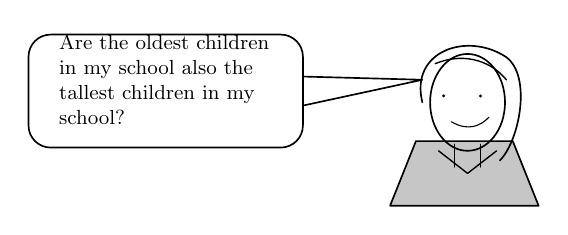
\begin{tikzpicture}[
						scale=0.82,
						every node/.style={font=\small, transform shape},
						line cap=round,
						line join=round
						]
						
						% Speech bubble
						\draw[line width=0.6pt, rounded corners=8pt]
						(0,0) rectangle (4.25,1.75);
						\draw[line width=0.6pt]
						(4.25,0.65) -- (6.1,1.05) -- (4.25,1.10);
						
						\node[align=left, anchor=west] at (0.35,1.05)
						{Are the oldest children\\in my school also the\\tallest children in my\\school?};
						
						% Simple student figure
						\begin{scope}[shift={(6.45,-0.15)}]
							% shoulders / uniform
							\fill[gray!45] (-0.85,-0.75) -- (1.45,-0.75) -- (1.05,0.25) -- (-0.45,0.25) -- cycle;
							\draw[line width=0.6pt] (-0.85,-0.75) -- (1.45,-0.75) -- (1.05,0.25) -- (-0.45,0.25) -- cycle;
							
							% neck and collar
							\draw[line width=0.5pt] (0.15,0.20) -- (0.15,-0.15);
							\draw[line width=0.5pt] (0.55,0.20) -- (0.55,-0.15);
							\draw[line width=0.5pt] (-0.1,0.10) -- (0.35,-0.25) -- (0.8,0.10);
							
							% head and hair
							\draw[line width=0.6pt] (0.35,0.85) ellipse (0.58 and 0.75);
							\draw[line width=0.6pt]
							(-0.35,0.85) .. controls (-0.55,1.65) and (0.35,1.95) .. (0.95,1.55)
							.. controls (1.35,1.25) and (1.15,0.25) .. (0.85,-0.05);
							\draw[line width=0.5pt]
							(-0.15,1.45) .. controls (0.35,1.65) and (0.75,1.45) .. (0.95,1.20);
							
							% face
							\fill (-0.02,0.95) circle (0.025);
							\fill (0.55,0.95) circle (0.025);
							\draw[line width=0.4pt] (0.10,0.55) .. controls (0.35,0.40) and (0.55,0.48) .. (0.68,0.62);
						\end{scope}
						
					\end{tikzpicture}
				\end{adjustbox}
			\end{center}
			
			\vspace{0.3cm}
			
			Write the \textbf{two sets} of data Safia needs to collect to answer her question.
			
			\vspace{0.35cm}
			
			\makebox[\linewidth]{\dotfill}
			
			\vspace{0.35cm}
			
			\makebox[\linewidth]{\dotfill} \QuestionMarks{1}
			
			\vspace{0.9cm}
			
			\item
			Draw a line to match the digital time to the equivalent time of day.
			
			\vspace{0.35cm}
			
			\begin{center}
				\begin{adjustbox}{max width=\linewidth}
					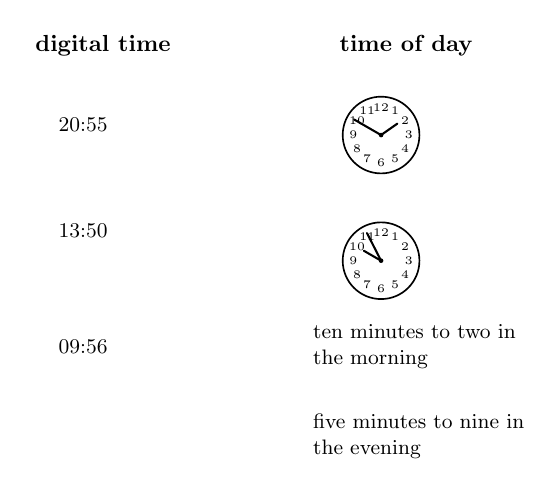
\begin{tikzpicture}[
						scale=0.84,
						every node/.style={font=\small, transform shape},
						line cap=round,
						line join=round
						]
						
						\node[font=\bfseries, anchor=west] at (0,5.8) {digital time};
						\node[font=\bfseries, anchor=west] at (4.6,5.8) {time of day};
						
						\node[anchor=west] at (0.35,4.6) {20:55};
						\node[anchor=west] at (0.35,3.0) {13:50};
						\node[anchor=west] at (0.35,1.25) {09:56};
						
						% Clock 1
						\begin{scope}[shift={(5.35,4.45)}]
							\draw[line width=0.6pt] (0,0) circle (0.58);
							\foreach \a/\n in {
								90/12,60/1,30/2,0/3,-30/4,-60/5,-90/6,
								-120/7,-150/8,180/9,150/10,120/11
							}
							\node[font=\tiny] at (\a:0.42) {\n};
							\draw[line width=0.75pt] (0,0) -- (150:0.47);
							\draw[line width=0.75pt] (0,0) -- (35:0.30);
							\fill (0,0) circle (0.035);
						\end{scope}
						
						% Clock 2
						\begin{scope}[shift={(5.35,2.55)}]
							\draw[line width=0.6pt] (0,0) circle (0.58);
							\foreach \a/\n in {
								90/12,60/1,30/2,0/3,-30/4,-60/5,-90/6,
								-120/7,-150/8,180/9,150/10,120/11
							}
							\node[font=\tiny] at (\a:0.42) {\n};
							\draw[line width=0.75pt] (0,0) -- (150:0.30);
							\draw[line width=0.75pt] (0,0) -- (117:0.47);
							\fill (0,0) circle (0.035);
						\end{scope}
						
						\node[align=left, anchor=west] at (4.2,1.25)
						{ten minutes to two in\\the morning};
						
						\node[align=left, anchor=west] at (4.2,-0.10)
						{five minutes to nine in\\the evening};
						
					\end{tikzpicture}
				\end{adjustbox}
			\end{center}
			
			\vspace{0.25cm}
			
			\QuestionMarks{1}
			
			\vspace{0.8cm}
			
			\item
			Eva has a measuring jug with a capacity of 1000 ml.
			
			\vspace{0.35cm}
			
			\begin{center}
				\begin{adjustbox}{max width=\linewidth}
					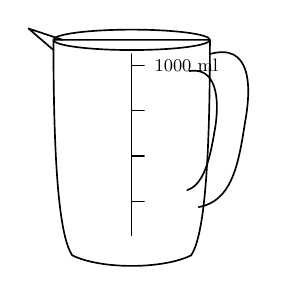
\begin{tikzpicture}[
						scale=0.72,
						every node/.style={font=\small, transform shape},
						line cap=round,
						line join=round
						]
						
						% Jug body
						\draw[line width=0.6pt]
						(0.95,0.20)
						.. controls (0.72,0.55) and (0.62,1.80) .. (0.62,4.00)
						-- (3.38,4.00)
						.. controls (3.38,1.80) and (3.28,0.55) .. (3.05,0.20)
						.. controls (2.55,-0.05) and (1.45,-0.05) .. (0.95,0.20)
						-- cycle;
						
						% Jug opening
						\draw[line width=0.6pt] (2.00,4.00) ellipse (1.38 and 0.18);
						
						% Spout
						\draw[line width=0.6pt]
						(0.62,3.82) -- (0.18,4.20) -- (0.78,4.00);
						
						% Handle
						\draw[line width=0.6pt]
						(3.38,3.75)
						.. controls (4.10,3.95) and (4.12,3.20) .. (4.00,2.55)
						.. controls (3.88,1.75) and (3.75,1.15) .. (3.18,1.05);
						\draw[line width=0.6pt]
						(3.02,3.45)
						.. controls (3.48,3.52) and (3.55,3.00) .. (3.48,2.50)
						.. controls (3.40,2.00) and (3.30,1.45) .. (2.98,1.35);
						
						% Measuring scale
						\draw[line width=0.5pt] (2.00,0.55) -- (2.00,3.75);
						\foreach \y in {1.15,1.95,2.75,3.55}
						\draw[line width=0.45pt] (2.00,\y) -- (2.22,\y);
						
						\node[anchor=west] at (2.28,3.55) {1000 ml};
						
					\end{tikzpicture}
				\end{adjustbox}
			\end{center}
			
			\vspace{0.35cm}
			
			She pours some water into the jug.
			
			The jug is now \textbf{three quarters} full.
			
			\vspace{0.35cm}
			
			Draw a line on the jug to show the level of the water. \QuestionMarks{1}
			
			\vspace{0.9cm}
			
			\item
			Here is a part of a sequence.
			
			\vspace{0.45cm}
			
			\[
			13
			\qquad\qquad
			15
			\qquad\qquad
			17
			\qquad\qquad
			19
			\]
			
			\vspace{0.35cm}
			
			The sequence continues in the same way.
			
			\vspace{0.35cm}
			
			Draw a ring around \textbf{all} the numbers which appear in the sequence.
			
			\vspace{0.65cm}
			
			\[
			51
			\qquad\qquad
			36
			\qquad\qquad
			74
			\qquad\qquad
			83
			\qquad\qquad
			37
			\]
			
			\vspace{0.25cm}
			
			\QuestionMarks{1}
			
			\vspace{0.8cm}
			
			\item
			Here is a table of fractions.
			
			\vspace{0.35cm}
			
			\begin{center}
				\begin{tabular}{|>{\centering\arraybackslash}p{1.75cm}|>{\centering\arraybackslash}p{2.25cm}|>{\centering\arraybackslash}p{2.55cm}|}
					\cline{2-3}
					\multicolumn{1}{c|}{} &
					\textbf{equivalent to \(\dfrac{1}{5}\)} &
					\textbf{not equivalent to \(\dfrac{1}{5}\)} \\
					\hline
					\(\dfrac{2}{10}\) & \rule{0pt}{0.9cm} & \\
					\hline
					\(\dfrac{3}{12}\) & \rule{0pt}{0.9cm} & \\
					\hline
					\(\dfrac{4}{15}\) & \rule{0pt}{0.9cm} & \\
					\hline
					\(\dfrac{5}{25}\) & \rule{0pt}{0.9cm} & \\
					\hline
				\end{tabular}
			\end{center}
			
			\vspace{0.35cm}
			
			Tick (\(\checkmark\)) to show if each fraction is equivalent to \(\dfrac{1}{5}\)
			or is not equivalent to \(\dfrac{1}{5}\). \QuestionMarks{1}
			
			\vspace{0.95cm}
			
			\item
			Lily chooses a number which rounds to 50\,000 when rounded to the nearest 10\,000.
			
			\vspace{0.45cm}
			
			Write a number Lily could choose.
			
			\vspace{0.8cm}
			
			\hfill \AnswerLine{4.2cm} \QuestionMarks{1}
			
			\vspace{0.8cm}
			
			\item
			Here is a bus timetable showing the time of buses from the Town Centre to Ashdown.
			
			\vspace{0.3cm}
			
			Each bus journey takes the same amount of time.
			
			\vspace{0.35cm}
			
			\begin{center}
				\begin{adjustbox}{max width=\linewidth}
					\begin{tabular}{|>{\raggedright\arraybackslash}p{2.35cm}|>{\centering\arraybackslash}p{1.55cm}|>{\centering\arraybackslash}p{1.55cm}|>{\centering\arraybackslash}p{1.55cm}|>{\centering\arraybackslash}p{1.55cm}|}
						\hline
						\textbf{Town Centre} & 12:15 & 13:30 & 15:45 & 15:52 \\
						\hline
						\textbf{West Town} & 12:26 & 13:41 & 15:56 & 16:03 \\
						\hline
						\textbf{Middleton} & 12:54 & 14:09 & 16:24 & 16:31 \\
						\hline
						\textbf{Ashdown} & 12:58 & 14:13 & 16:28 & 16:35 \\
						\hline
					\end{tabular}
				\end{adjustbox}
			\end{center}
			
			\vspace{0.45cm}
			
			\textbf{(a)}\quad
			Calculate the length of time for the bus journey from West Town to Ashdown.
			
			Write the time in minutes.
			
			\vspace{0.75cm}
			
			\hfill \AnswerLine{3.6cm}\quad minutes \QuestionMarks{1}
			
			\vspace{0.9cm}
			
			\textbf{(b)}\quad
			Blessy travels by bus from the Town Centre to Middleton.
			
			She must be in Middleton by 16:30.
			
			\vspace{0.45cm}
			
			Write the time of the latest bus she can take from the town centre.
			
			\vspace{0.75cm}
			
			\hfill \AnswerLine{3.6cm} \QuestionMarks{1}
			
			\vspace{0.8cm}
			
			\item
			Here are some numbers.
			
			\vspace{0.45cm}
			
			\[
			3
			\qquad\qquad
			6
			\qquad\qquad
			14
			\qquad\qquad
			18
			\qquad\qquad
			21
			\]
			
			\vspace{0.45cm}
			
			\textbf{(a)}\quad
			Write the number which is not a multiple of 3.
			
			\vspace{0.65cm}
			
			\hfill \AnswerLine{3.8cm} \QuestionMarks{1}
			
			\vspace{0.9cm}
			
			\textbf{(b)}\quad
			Write the number which is not a factor of 42.
			
			\vspace{0.65cm}
			
			\hfill \AnswerLine{3.8cm} \QuestionMarks{1}
			
			\vspace{0.9cm}
			
			\item
			Here is a bag of 28 sweets.
			
			\vspace{0.35cm}
			
			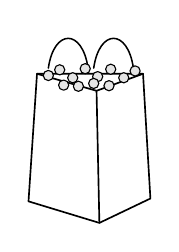
\begin{tikzpicture}[
				scale=0.72,
				every node/.style={font=\small, transform shape},
				line cap=round,
				line join=round
				]
				
				% Bag body
				\draw[line width=0.6pt]
				(0,0) -- (1.25,-0.38) -- (2.15,0.05) -- (2.02,2.25) -- (0.15,2.25) -- cycle;
				
				\draw[line width=0.6pt] (0.15,2.25) -- (1.20,1.95) -- (2.02,2.25);
				\draw[line width=0.6pt] (1.20,1.95) -- (1.25,-0.38);
				
				% Handles
				\draw[line width=0.55pt]
				(0.35,2.35) .. controls (0.45,3.05) and (0.95,3.05) .. (1.05,2.35);
				\draw[line width=0.55pt]
				(1.15,2.35) .. controls (1.25,3.05) and (1.75,3.05) .. (1.85,2.35);
				
				% Sweets
				\foreach \x/\y in {
					0.35/2.22, 0.55/2.32, 0.78/2.18, 1.00/2.34,
					1.22/2.20, 1.45/2.33, 1.68/2.18, 1.88/2.30,
					0.62/2.05, 0.88/2.03, 1.15/2.08, 1.42/2.04
				}
				{
					\draw[line width=0.4pt, fill=gray!20] (\x,\y) circle (0.09);
				}
				
			\end{tikzpicture}
			
			\vspace{0.45cm}
			
			Calculate \(\dfrac{3}{4}\) of the number of sweets in the bag.
			
			\vspace{0.8cm}
			
			\hfill \AnswerLine{3.8cm}\quad sweets \QuestionMarks{1}
			
			\vspace{0.8cm}
			
			\item
			Here are some fractions and percentages.
			
			\vspace{0.35cm}
			
			\begin{center}
				\begin{adjustbox}{max width=\linewidth}
					\begin{tikzpicture}[
						scale=0.85,
						every node/.style={font=\small, transform shape},
						line cap=round,
						line join=round
						]
						
						\node[font=\bfseries] at (1.7,5.7) {fraction};
						\node[font=\bfseries] at (6.8,5.7) {percentage};
						
						\node at (1.7,4.8) {\(\dfrac{1}{4}\)};
						\node at (1.7,3.8) {\(\dfrac{3}{4}\)};
						\node at (1.7,2.8) {\(\dfrac{1}{2}\)};
						\node at (1.7,1.8) {\(\dfrac{25}{100}\)};
						\node at (1.7,0.8) {\(\dfrac{1}{100}\)};
						
						\node at (6.8,4.25) {1\%};
						\node at (6.8,3.25) {25\%};
						\node at (6.8,2.25) {50\%};
						\node at (6.8,1.25) {75\%};
						
					\end{tikzpicture}
				\end{adjustbox}
			\end{center}
			
			\vspace{0.35cm}
			
			Draw a line to match each fraction to the equivalent percentage. \QuestionMarks{2}
			
			\vspace{0.8cm}
			
			\item
			Priya sorts some 3D shapes on to a Carroll diagram.
			
			\vspace{0.35cm}
			
			\begin{center}
				\begin{adjustbox}{max width=\linewidth}
					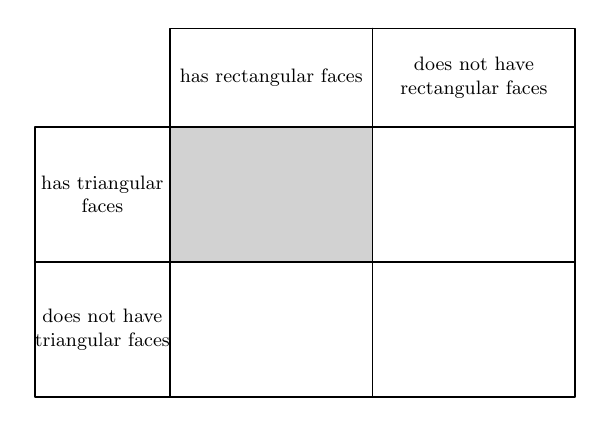
\begin{tikzpicture}[
						scale=0.78,
						every node/.style={font=\small, transform shape},
						line cap=round,
						line join=round
						]
						
						% Column headers
						\draw[line width=0.6pt] (2.2,4.4) rectangle (8.8,6.0);
						\draw[line width=0.6pt] (5.5,4.4) -- (5.5,6.0);
						
						% Body and row headers
						\draw[line width=0.6pt] (0,0) rectangle (8.8,4.4);
						\draw[line width=0.6pt] (2.2,0) -- (2.2,4.4);
						\draw[line width=0.6pt] (5.5,0) -- (5.5,4.4);
						\draw[line width=0.6pt] (0,2.2) -- (8.8,2.2);
						
						% Shaded area
						\fill[gray!35] (2.2,2.2) rectangle (5.5,4.4);
						\draw[line width=0.6pt] (2.2,2.2) rectangle (5.5,4.4);
						
						% Header text
						\node[align=center] at (3.85,5.2) {has rectangular faces};
						\node[align=center] at (7.15,5.2) {does not have\\rectangular faces};
						
						% Row label text
						\node[align=center] at (1.1,3.3) {has triangular\\faces};
						\node[align=center] at (1.1,1.1) {does not have\\triangular faces};
						
					\end{tikzpicture}
				\end{adjustbox}
			\end{center}
			
			\vspace{0.35cm}
			
			\textbf{(a)}\quad Tick (\(\checkmark\)) the section where Priya places the cuboid. \QuestionMarks{1}
			
			\vspace{0.7cm}
			
			\textbf{(b)}\quad Sketch a shape that Priya could place in the shaded area.
			
			\vspace{4.2cm}
			
			\QuestionMarks{1}
			
			\vspace{0.8cm}
			
			\item
			Here is a rectangle drawn on a grid of squares.
			
			\vspace{0.35cm}
			
			\begin{center}
				\begin{adjustbox}{max width=\linewidth}
					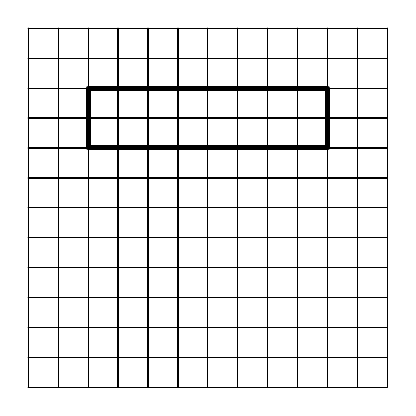
\begin{tikzpicture}[
						scale=0.38,
						line cap=round,
						line join=round
						]
						
						% Grid
						\draw[step=1, line width=0.45pt] (0,0) grid (12,12);
						
						% Given rectangle: 8 by 2
						\draw[line width=1.8pt] (2,8) rectangle (10,10);
						
					\end{tikzpicture}
				\end{adjustbox}
			\end{center}
			
			\vspace{0.35cm}
			
			Draw a \textbf{square} with the same perimeter as the rectangle. \QuestionMarks{1}
			
			\vspace{0.8cm}
			
			\item
			The table shows the number of visitors to local parks on Friday and Saturday.
			
			\vspace{0.35cm}
			
			\begin{center}
				\begin{adjustbox}{max width=\linewidth}
					\begin{tabular}{|>{\raggedright\arraybackslash}p{2.5cm}|>{\centering\arraybackslash}p{2.6cm}|>{\centering\arraybackslash}p{2.6cm}|}
						\hline
						\textbf{name of park} &
							\begin{tabular}[c]{@{}c@{}}\textbf{number of visitors}\\\textbf{on Friday}\end{tabular} &
							\begin{tabular}[c]{@{}c@{}}\textbf{number of visitors}\\\textbf{on Saturday}\end{tabular} \\
						\hline
						Animal Park & 562 & 421 \\
						\hline
						Downtown Park & 357 & 243 \\
						\hline
						Cinema Park & 653 & 322 \\
						\hline
						Magical Park & 248 & 352 \\
						\hline
					\end{tabular}
				\end{adjustbox}
			\end{center}
			
			\vspace{0.35cm}
			
			Tick (\(\checkmark\)) the box to show if the statement is true or false.
			
			\vspace{0.35cm}
			
			\begin{center}
				\begin{adjustbox}{max width=\linewidth}
					\begin{tabular}{|>{\raggedright\arraybackslash}p{6.2cm}|>{\centering\arraybackslash}p{0.95cm}|>{\centering\arraybackslash}p{0.95cm}|}
						\cline{2-3}
						\multicolumn{1}{c|}{} & \textbf{true} & \textbf{false} \\
						\hline
						More people visit Animal Park than Cinema Park on Friday. &
						\rule{0pt}{1.0cm} & \\
						\hline
						Both Downtown Park and Magical Park have the same total number of visitors on Friday and Saturday. &
						\rule{0pt}{1.25cm} & \\
						\hline
						Animal Park has the greatest \textbf{total} number of visitors. &
						\rule{0pt}{1.0cm} & \\
						\hline
						Cinema Park was the \textbf{least} popular park on Saturday. &
						\rule{0pt}{1.0cm} & \\
						\hline
					\end{tabular}
				\end{adjustbox}
			\end{center}
			
			\vspace{0.25cm}
			
			\QuestionMarks{2}
			
			\vspace{0.8cm}
			
		\end{enumerate}
	\end{multicols}
\end{document}
